\appendix
\addtocontents{toc}{%
  \protect\vspace{1em}%
  \protect\noindent \bfseries \appendixtocname\protect\par
  \protect\vspace{-.5em}%
 }
 \renewcommand{\chaptername}{\appendixname}

\begin{appendices}

\chapter{Appendix A}

\section{Socket.IO Implementation Script}
\label{server:socket}

\begin{lstlisting}[caption={socket.js on Application Server},label={code:server_socket}]
SocketManager.prototype.listen = function(server){
  ...
  io = socketio.listen(server);
  io.sockets.on('connection', _handlerSocket);
  _handlerSip();
}

function _handlerSocket(socket) {
  var delivery = dl.listen(socket);
    ...
  socket.on('sip',function (data){
    switch(data.type){
      case 'register':
        if(data.username != ""){
          gw.register(data.content.browserClient,function(result){
            socket.emit('sip',result);
          });
        }
        break;
      ...
    }
  });

  socket.on('webrtc', function (data) {
        ...  
    });

  socket.on('message',function(data){
    ...
  });

  socket.on('disconnect', function() {
    ...
  });

  delivery.on('receive.success',function(file){
    ...
    fs.writeFile(file.name,file.buffer, function(err){
      if(err){
        console.log('File could not be saved.');
      }else{
        console.log('File saved.');
        _und.each(clients,function(client,key){
          if(sendingClient.conf_id && client.conf_id == sendingClient.conf_id && client.username != sendingClient.username){
            ...
            client.delivery.send({
              name: file.name,
              path : './' + file.name
            });

          }
        });

        fs.unlink('./' + file.name);
      };
    });
  });

}
\end{lstlisting}

\section{SIP Implementation Script}
\label{server:sip}

\begin{lstlisting}[caption={sip.js on Application Server},label={code:sipjs}]
function SipGateway(config){
	EventEmitter.call(this);
	this.config = config || {
		realm: os.hostname(),
		hostPublicAddress: 'xxx.xxx.xxx.xxx',
		hostPort: 5060,
		hostBranch: 'z9hG4bK-' + uuid.v1()
	};
	this.init();
}

util.inherits(SipGateway, EventEmitter);

function rstring() {
	return Math.floor(Math.random() * 1e6).toString();
}

function unq(a) {
  if(a && a[0] === '"' && a[a.length-1] === '"')
    return a.substr(1, a.length - 2);
  return a;
}

function createRegister(user){
	return {
	  method: 'REGISTER',
	  uri: 'sip:' + user.hostname,
	  headers:
	  {
	  	'call-id': user.callid,
	  	cseq: {method: 'REGISTER', seq: ++user.seq},
	  	from: {name: '', uri: 'sip:' + user.name + '@' + user.hostname, params: { tag: user.tag }},
	    to: {name: '', uri: 'sip:' + user.name + '@' + user.hostname},
	    expires: 3600,
	  	contact:  [{
      	uri: 'sip:' + user.name + '@'+ hostPublicAddress + ':' + hostPort
      }]

	  }
	}
}

function createInvite(client, to){
  return {
		method: 'INVITE',
		uri: 'sip:' + to + '@'+  client.hostname,
		headers: {
			'call-id': client.callid,
			cseq: {
				method: 'INVITE',
				seq: 1
			},
			from: {
        name: '',
				uri: 'sip:' + client.name + '@'+ client.hostname,
				params: {
					tag: client.tag
				}
			},
			to: {
				uri: 'sip:' + to +'@'+ client.hostname
			},
			expires: 3600,
			contact: [{name: '',
				uri: 'sip:' + client.name + '@'+ hostPublicAddress + ':' + hostPort
			}]
		}
  }
}

function createInviteACK(rs,client,sdp){
	var uri = rs.headers.contact[0].uri.split(';');
	if(uri[0].split(':').length != 3){
		uri[0] = uri[0] + ':5060';
	}
	return {
		method: 'ACK',
		uri: uri[0],
		headers: {
			'call-id': rs.headers['call-id'],
			cseq: {
				method: 'ACK',
				seq: rs.headers.cseq.seq
			},
			from: rs.headers.from,
			to: rs.headers.to,
			authorization: client.inviteAuth,
			'content-type': 'application/sdp'
		},
		content: sdp
	}
}

function createAnswerOK(rq,client,sdp){
	var rs = sip.makeResponse(rq, 200, 'OK');

	rs.headers.to.params.tag = client.tag;

	rs.headers.contact = [{
  	uri: 'sip:' + client.name + '@'+ hostPublicAddress + ':' + hostPort
  }];

  rs.headers.expires = 3600;
	rs.headers['content-type'] = 'application/sdp';
	//rs.headers['Allow'] = 'INVITE, ACK, CANCEL, BYE, NOTIFY, REFER, MESSAGE, OPTIONS, INFO, SUBSCRIBE';
	//rs.headers['Supported'] = 'replaces';
	rs.content = sdp;

	return rs;
}

function createBye(client){
	var to,from;

	if(client.name != sip.parseUri(client.from.uri).user){
		from = client.to;
		to = client.from;
	}else{
		from = client.from;
		to = client.to;
	}

	return {
	  method: 'BYE',
	  uri: 'sip:' + client.hostname + ':5060',
	  headers:
	  {
	  	'call-id': client.callid,
	  	cseq: {method: 'BYE', seq: 3},
	  	from: from,
	    to: to,
	  	contact:  [{
      	uri: 'sip:' + client.name + '@'+ hostPublicAddress + ':' + hostPort
      }],
      authorization: client.authorization

	  }
	}
}

function createCancel (client,to) {

	//util.debug("createCancel: \n" + util.inspect(client, false, null));

	return {
	  method: 'CANCEL',
	  uri: 'sip:' + to + '@' + client.hostname,
	  headers:
	  {
	  	'call-id': client.callid,
	  	cseq: {method: 'CANCEL', seq: 2},
			from: {
        name: '',
				uri: 'sip:' + client.name + '@'+ client.hostname,
				params: {
					tag: client.tag
				}
			},
			to: {
				uri: 'sip:' + to +'@'+ client.hostname
			},
      authorization: client.inviteAuth

	  }
	}
}

function createSMS(client,to,msg){

	return {
		method: 'MESSAGE',
		uri: 'sip:' + to + '@'+  client.hostname,
		headers: {
			'call-id': client.callid,
			cseq: {
				method: 'MESSAGE',
				seq: 1
			},
			from: {
        name: '',
				uri: 'sip:' + client.name + '@'+ client.hostname,
				params: {
					tag: client.tag
				}
			},
			to: {
				uri: 'sip:' + to +'@'+ client.hostname
			},
			authorization: client.authorization,
			'content-type': 'text/plain',
			'content-length': msg.length
		},
		content: msg
	}

}

SipGateway.prototype.init = function () {
	var self = this;
	realm = this.config.realm;
	hostPublicAddress = this.config.hostPublicAddress;
	hostPort = this.config.hostPort;
	hostBranch = this.config.hostBranch;
	registry = {};

	sip.start({
		port: hostPort,
	  logger: {
	    send: function(message, address) { util.debug("send\n" + util.inspect(message, false, null)); },
	    recv: function(message, address) { util.debug("recv\n" + util.inspect(message, false, null)); }
	  },
	  publicAddress: hostPublicAddress,
	  tcp: false
	},
	function(rq) {

	  try {
	    if(rq.method === 'REGISTER') {
	      util.debug('request register');
	      //looking up user info
	      var username = sip.parseUri(rq.headers.to.uri).user;

	      registry[username] = rq.headers.contact;

	      //var rs = sip.makeResponse(rq, 200, 'Ok');
	      //rs.headers.contact = rq.headers.contact;
	      //sip.send(rs);
	    }
	    else if(rq.method === 'INVITE') {

	      var username = sip.parseUri(rq.uri).user;
	      var contact = registry[username];

	      var rs = sip.makeResponse(rq, 100, 'Trying');
	      sip.send(rs);

	      if(contact) {
	      	registry[username].callid = rq.headers['call-id'];
	      	registry[username].tag = rstring();
	      	registry[username].from = rq.headers.from;
					registry[username].to = rq.headers.to;

	        self.emit('SIPREMOTE',{
	        	type: 'INVITE',
	        	content:{
	        		fromNumber: sip.parseUri(rq.headers.from.uri).user,
	        		toNumber: username,
	        		inviteRequest: rq
	        	}
	        });

	        rs = sip.makeResponse(rq, 180, 'Ringing');
					sip.send(rs);
	      }
	      else {
	        sip.send(sip.makeResponse(rq, 404, 'Not Found'));
	      }

	    }
	    else if(rq.method === 'BYE'){
	    	var endNumber = sip.parseUri(rq.headers.to.uri).user;
	    	var sipNumber = sip.parseUri(rq.headers.from.uri).user;
	    	//console.log(endNumber);
	    	var rs = sip.makeResponse(rq, 200, 'Ok');
	    	sip.send(rs);
	    	self.emit('SIPREMOTE', {
	    		type: 'BYE',
	    		content:{
	    			endNumber: endNumber,
	    			sipNumber: sipNumber
	    		}
	    	});
	    }
	    else if(rq.method === 'ACK'){
	    	util.debug("sip ACK: \n" + util.inspect(rq, false, null));

				var username = sip.parseUri(rq.uri).user;
	    	registry[username].answerAcked = true;
	    }
	    else if(rq.method === 'CANCEL'){
	    	var endNumber = sip.parseUri(rq.headers.to.uri).user;
	    	var sipNumber = sip.parseUri(rq.headers.from.uri).user;
	    	//console.log(endNumber);
	    	var rs = sip.makeResponse(rq, 200, 'Ok');
	    	sip.send(rs);
	    	self.emit('SIPREMOTE', {
	    		type: 'CANCEL',
	    		content:{
	    			endNumber: endNumber,
	    			sipNumber: sipNumber
	    		}
	    	});
	    }
	    else {
	      sip.send(sip.makeResponse(rq, 405, 'Method Not Allowed'));
	    }
	  } catch(e) {
	    util.debug(e);
	    util.debug(e.stack);

	    sip.send(sip.makeResponse(rq, 500, "Server Internal Error"));
	  }

	});


}

function _register(client,callback){

	var rq = createRegister(client);

	sip.send(rq,function(rs){

		if(rs.status === 401){
			var user = client;
			var creds = { user: user.name, password: user.password, realm: user.hostname };

			rq.headers['cseq'].seq++;
	    rq.headers.via.shift();
	    rq.headers['call-id'] = user.callid;
	    client.seq = rq.headers['cseq'].seq;

	    digest.signRequest(creds, rq, rs, creds);
			sip.send(rq,function(rs){
				if(rs.status === 200){

					client.authorization = rq.headers.authorization;

					if(!client.registerTimer){
						client.registerTimer = setInterval(function(){
							console.log('register timer');
							_register(client);
						},parseInt(rs.headers.expires)*1000);
					}

					if(callback){
						callback({type: 'register',msg: 'success'});
					}
				}else{
					if(callback){
						callback({type: 'register',msg: 'failed'});
					}
				}
			});
		}else if(rs.status === 200){
			if(callback){
				callback({type: 'register',msg: 'success'});
			}
		}

	});

}


SipGateway.prototype.register = function(client,callback){
	registry[client.name] = {
		name : client.name,
		password : client.pwd,
		hostname : client.host,
		callid : rstring() + '@' + hostPublicAddress,
		tag: rstring(),
		registerTimer: null,
		seq: 0
	};

	_register(registry[client.name],callback);
}

SipGateway.prototype.unregister = function(username){

	clearInterval(registry[username].registerTimer);

}

SipGateway.prototype.invite = function(from,to,callback){
	var self = this;
	registry[from].callid = rstring() + '@' + hostPublicAddress;
	registry[from].tag = rstring();

	var client = registry[from];

	var invite_rq = createInvite(client,to);

	client.answerAcked = false;

	sip.send(invite_rq,function(rs){
		if(rs.status === 100){
			client.answerAcked = false;
		}else if(rs.status === 180){
			client.answerAcked = false;
		}
		else if(rs.status === 401){
			//util.debug("invite response: \n" + util.inspect(rs, false, null));

			//util.debug("invite before digest: \n" + util.inspect(invite_rq, false, null));

			invite_rq.headers['cseq'].seq++;
	    invite_rq.headers.via.shift();
	    invite_rq.headers['call-id'] = client.callid;

	    var creds = { user: client.name, password: client.password, realm: unq(rs.headers['www-authenticate'][0].realm) };

			var new_invite_req = digest.signRequest(creds, invite_rq, rs, creds);
			registry[from].inviteAuth = new_invite_req.headers.authorization;
			registry[from].invite_req = new_invite_req;
			//util.debug("invite to be sent: \n" + util.inspect(invite_rq, false, null));

			sip.send(new_invite_req,function(rs){

				if(rs.status === 200){
					//util.debug("second invite response: \n" + util.inspect(rs, false, null));
					if(!client.answerAcked){
						client.answerAcked = true;
						callback(rs);
					}
				}else if(rs.status === 100){

					self.emit('SIPREMOTE', {
		    		type: 'TRYING',
		    		content:{
		    			clientNumber: from,
		    			sipNumber: to
	    			}
		    	});

				}else if(rs.status === 180){

					self.emit('SIPREMOTE', {
		    		type: 'RINGING',
		    		content:{
		    			clientNumber: from,
		    			sipNumber: to
	    			}
		    	});

				}else if(rs.status === 486){

					self.emit('SIPREMOTE', {
		    		type: 'BUSY',
		    		content:{
		    			clientNumber: from,
		    			sipNumber: to
	    			}
		    	});

				}
			});
		}else if(rs.status === 200)
			if(!client.answerAcked){
				client.answerAcked = true;
				callback(rs);
			}
	});
}

SipGateway.prototype.ackInvite = function(from,rs,xmsSDP,callback){
	var client = registry[from];
	var ack = createInviteACK(rs,client,xmsSDP);

	util.debug("ack message: \n" + util.inspect(ack, false, null));

	client.from = ack.headers.from;
	client.to = ack.headers.to;

	sip.send(ack);

	callback();//not really callback since there is no response for ack message from server

}

SipGateway.prototype.sendTrying = function(rq){
	var rs = sip.makeResponse(rq, 100, 'Trying');
	sip.send(rs);
}

SipGateway.prototype.sendRing = function(to,rq){
	var client = registry[to];

	var rs = sip.makeResponse(rq, 180, 'Ringing');

	rs.headers.to.params.tag = registry[to].tag;

	sip.send(rs);
}

SipGateway.prototype.sendAnswer = function(to,rq,xmsSDP,callback){
	var client = registry[to];
	registry[to].answerAcked = false;

	//var rs = sip.makeResponse(rq, 100, 'Trying');
	//sip.send(rs);

	//rs = sip.makeResponse(rq, 180, 'Ringing');
	//sip.send(rs);

	var ok = createAnswerOK(rq,client,xmsSDP);

	sip.send(ok);

	callback();

}

SipGateway.prototype.sendBye = function(number,callback){
	var client = registry[number];

	var bye = createBye(client);

	sip.send(bye,function(rs){
		if(rs.status === 200){
			callback();
		}
	});
}

SipGateway.prototype.sendCancel = function(from,to,callback){
	var client = registry[from];

	var cancel = createCancel(client,to);

	util.debug("sip:Cancel: \n" + util.inspect(cancel, false, null));

	sip.send(cancel,function(rs){
		if(rs.status === 200){
			callback();
		}
	});
}

SipGateway.prototype.sendBusy = function(rq,callback){

	var busy = sip.makeResponse(rq, 486, 'Busy');

	sip.send(busy,function(rs){
		if(rs.status === 200){
			callback();
		}
	});
}

SipGateway.prototype.sendSMS = function(from,to,msg,callback){

	var client = registry[from];

	var sms = createSMS(client,to,msg);

	sip.send(sms,function(rs){
		if(rs.status === 200){
			callback();
		}
	});

}

module.exports.SipGateway = SipGateway;
\end{lstlisting}


\section{XMS Implementation Script}
\label{server:xms}

\begin{lstlisting}[caption={xms.js on Application Server},label={code:xms}]
XmsManager.prototype.createXMSCall = function(data,callback){
  var requestContent = "<web_service version=\"1.0\">";
  requestContent += "\n<call";
  requestContent += " sdp=\"" + data.sdp.replace(/\r\n/g, "&#xA;") + "\"";
  if(data.callType === 'webrtc'){
    requestContent += " encryption=\"dtls\"" + " ice=\"yes\"";
  }
  requestContent += " media=\"audiovideo\"" + " signaling= \"no\"/>";
  requestContent += "\n</web_service>";

  console.log(requestContent);
  var req = http.request({
    host: xmsAddress,
    port: xmsPort,
    method: 'POST',
    path: xmsPath + 'calls?appid=' + xmsAppId,
    headers: {
      'Accept' : 'application/xml',
      'Content-Type' : 'application/xml',
      'Content-Length' : requestContent.length
    }
  }, function(res) {
    var resData = '';
    console.log('createXMSCall:STATUS: ' + res.statusCode);
    console.log('createXMSCall:HEADERS: ' + JSON.stringify(res.headers));
    res.setEncoding('utf8');

    res.on('data', function (chunk) {
      resData += chunk;
    }).on('end', function() {
      if(resData != ''){
        xmlparser.parseString(resData,function(err,result){
          var xmsSdp = result['web_service']['call_response'][0]['$'].sdp;
          var id = result['web_service']['call_response'][0]['$'].identifier;

          var regex = new RegExp(xmsAddress,"g");
          pub_xmsSdp = xmsSdp.replace(regex,xmsPublicAddress);
          console.log('after create call sdp: ' + pub_xmsSdp);

          callback(pub_xmsSdp.replace(/\n/g,"\r\n"),id);
        });
      }
    });
  });

  req.write(requestContent);
  req.end();
}

XmsManager.prototype.joinXMSCall = function(call,callback){
  var requestContent = "<web_service version=\"1.0\">";
  requestContent += "\n<call>";
  requestContent += "\n<call_action>";
  requestContent += "\n<join call_id=\"" + call.remote_identifier + "\"/>";
  requestContent += "\n</call_action>";
  requestContent += "\n</call>";
  requestContent += "\n</web_service>";

  var joinPath = xmsPath + 'calls/' + call.local_identifier + '?appid=' + xmsAppId;

  var req = http.request({
    host: xmsAddress,
    port: xmsPort,
    method: 'PUT',
    path: joinPath,
    headers: {
      'Accept' : 'application/xml',
      'Content-Type' : 'application/xml',
      'Content-Length' : requestContent.length
    }
  }, function(res) {
    var resData = '';
    console.log('joinXMSCall:STATUS: ' + res.statusCode);
    console.log('joinXMSCall:HEADERS: ' + JSON.stringify(res.headers));
    res.setEncoding('utf8');

    res.on('data', function (chunk) {
      resData += chunk;
    }).on('end', function() {
      if(resData != ''){
        callback(resData);
      }
    });
  });

  req.write(requestContent);
  req.end();
}

XmsManager.prototype.updateLocalSDP = function(newSDP,call,callback){
  var requestContent = "<web_service version=\"1.0\">";
  requestContent += "\n<call" + " sdp=\""
    + newSDP.replace(/\r\n/g, "&#xA;") + "\"";
  requestContent += " encryption=\"dtls\"" + " ice=\"yes\"";
  requestContent += " media=\"audiovideo\"" + " signaling= \"no\"/>";
  requestContent += "\n</web_service>";

  var updatePath = xmsPath + 'calls/' + call.local_identifier + '?appid=' + xmsAppId;
  //console.log('update request content: '+ requestContent);

  var req = http.request({
    host: xmsAddress,
    port: xmsPort,
    method: 'PUT',
    path: updatePath,
    headers: {
      'Accept' : 'application/xml',
      'Content-Type' : 'application/xml',
      'Content-Length' : requestContent.length
    }
  }, function(res) {
    var resData = '';
    console.log('updateLocalSDP:STATUS: ' + res.statusCode);
    console.log('updateLocalSDP:HEADERS: ' + JSON.stringify(res.headers));
    res.setEncoding('utf8');

    res.on('data', function (chunk) {
      resData += chunk;
    }).on('end', function() {
      if(resData != ''){
        xmlparser.parseString(resData,function(err,result){
          var xmsSdp = result['web_service']['call_response'][0]['$'].sdp;

          //console.log('after update sdp: ' + xmsSdp);
          if(xmsSdp){
            xmsSdp = xmsSdp.replace(xmsAddress,xmsPublicAddress);
            callback(xmsSdp.replace(/\n/g,"\r\n"));
          }else{
            callback(null);
          }

        });
      }
    });
  });

  req.write(requestContent);
  req.end();
}

XmsManager.prototype.createConference = function(options,callback){
  var requestContent = "<web_service version=\"1.0\">";
  requestContent += "\n<conference type=\"" + options.type + "\" max_parties=\"" + options.max_p + "\" reserve=\"" + options.reserve + "\"";
  requestContent += " layout=\"" + options.layout + "\" caption=\"" + options.caption + "\"";
  requestContent += " caption_duration=\"30s\" beep=\"yes\" clamp_dtmf=\"yes\" auto_gain_control=\"yes\" echo_cancellation=\"yes\" />";
  requestContent += "\n</web_service>"

  //console.log("createConference: " + requestContent);
  var createConfPath = xmsPath + '/conferences?appid=' + xmsAppId;
  //console.log("createConference path: " + createConfPath);

  var req = http.request({
    host: xmsAddress,
    port: xmsPort,
    method: 'POST',
    path: createConfPath,
    headers: {
      'Accept' : 'application/xml',
      'Content-Type' : 'application/xml',
      'Content-Length' : requestContent.length
    }
  }, function(res) {
    var resData = '';
    console.log('createConference:STATUS: ' + res.statusCode);
    console.log('createConference:HEADERS: ' + JSON.stringify(res.headers));
    res.setEncoding('utf8');

    res.on('data', function (chunk) {
      resData += chunk;
    }).on('end', function() {
      if(resData != ''){
        xmlparser.parseString(resData,function(err,result){
          var conf_id = result['web_service']['conference_response'][0]['$'].identifier;

          callback(conf_id);

        });
      }
    });
  });

  req.write(requestContent);
  req.end();
}

XmsManager.prototype.joinConference = function(call_id,conf_id,options,callback){
  var requestContent = "<web_service version=\"1.0\">";
  requestContent += "\n<call>";
  requestContent += "\n<call_action>";
  requestContent += "\n<add_party conf_id=\"" + conf_id + "\" caption=\"" + options.caption + "\"";
  requestContent += " region=\"" + options.region + "\" audio=\"" + options.audio + "\" video=\"" + options.video + "\" />";
  requestContent += "\n</call_action>";
  requestContent += "\n</call>";
  requestContent += "\n</web_service>";

  console.log("joinConference: " + requestContent);
  var joinPath = xmsPath + 'calls/' + call_id + '?appid=' + xmsAppId;

  var req = http.request({
    host: xmsAddress,
    port: xmsPort,
    method: 'PUT',
    path: joinPath,
    headers: {
      'Accept' : 'application/xml',
      'Content-Type' : 'application/xml',
      'Content-Length' : requestContent.length
    }
  }, function(res) {
    var resData = '';
    console.log('joinConference:STATUS: ' + res.statusCode);
    console.log('joinConference:HEADERS: ' + JSON.stringify(res.headers));
    res.setEncoding('utf8');

    res.on('data', function (chunk) {
      resData += chunk;
    }).on('end', function() {
      if(resData != '' && res.statusCode === 200){

        callback('yes');

      }
    });
  });

  req.write(requestContent);
  req.end();
}

XmsManager.prototype.deleteXMSCall = function(callId,callback){
  var deletePath = xmsPath + 'calls/' + callId + '?appid=' + xmsAppId;

  var req = http.request({
    host: xmsAddress,
    port: xmsPort,
    method: 'DELETE',
    path: deletePath
  },function(res){
    console.log('deleteXMSCall:STATUS: ' + res.statusCode);
    console.log('deleteXMSCall:HEADERS: ' + JSON.stringify(res.headers));
    res.setEncoding('utf8');

    callback(res);
  });

  req.end();
}

XmsManager.prototype.deleteXMSConference = function(confId,callback){

  var deletePath = xmsPath + 'conferences/' + confId + '?appid=' + xmsAppId;

  var req = http.request({
    host: xmsAddress,
    port: xmsPort,
    method: 'DELETE',
    path: deletePath
  },function(res){
    console.log('deleteXMSConference:STATUS: ' + res.statusCode);
    console.log('deleteXMSConference:HEADERS: ' + JSON.stringify(res.headers));
    res.setEncoding('utf8');

    callback(res);
  });

  req.end();

}

module.exports.XmsManager = XmsManager;
\end{lstlisting}

\section{MSG Implementation Script}
\label{server:msg}

\begin{lstlisting}[caption={msg.js on Application Server},label={code:msg}]
MsgManager.prototype.login = function(loginDto,success,fail){

	var loginStr = JSON.stringify(loginDto);

	var options = {
		host: msgRestUrl,
		path: '/your/url/here/loginWithDto',
		method : 'POST',
		headers: {
			"Accept" : "application/json",
			"Content-Type" : "application/json",
			'Content-Length' : loginStr.length
		}
	};

	var req = https.request(options, function(res) {
		var resData = '';
	  console.log("MSG:LOGIN:statusCode: ", res.statusCode);
	  console.log("MSG:LOGIN:headers: ", res.headers);
	  res.setEncoding('utf8');

	  res.on('data', function (chunk) {
      resData += chunk;
    }).on('end', function() {
    	if(resData != ''){
    		var jsonObject = JSON.parse(resData);
    		if(jsonObject.code === 200){
    			success(jsonObject,res.headers['set-cookie'][0]);
    		}else{
    			fail(jsonObject);
    		}
    	}
    });
	});

	req.write(loginStr);
	req.end();

	req.on('error', function(e) {
	  console.error(e);
	  fail(e);
	});

}

MsgManager.prototype.sendSMS = function(organization,login,cookie,msgObj,success,fail){

	var msgStr = JSON.stringify(msgObj);
	console.log(msgObj);

	var options = {
		host: msgRestUrl,
		path: '/your/url/here/sms',
		method : 'POST',
		headers : {
			"Accept" : "application/json",
			"Content-Type" : "application/json",
			"organization" : organization,
			"login" : login,
			"Cookie" : cookie,
			'Content-Length' : msgStr.length
		}
	};

	var req = https.request(options, function(res) {
		var resData = '';
	  console.log("MSG:SENDSMS:statusCode: ", res.statusCode);
	  console.log("MSG:SENDSMS:headers: ", res.headers);
	  res.setEncoding('utf8');

	  res.on('data', function (chunk) {
      resData += chunk;
    }).on('end', function() {
    	if(resData != ''){
    		var jsonObject = JSON.parse(resData);
    		console.log('MSG:SENDSMS:jsonObject:',jsonObject);
    		if(jsonObject.code === 200){//TODO: check report values as true
    			success();
    		}else{
    			fail();
    		}
    	}
    });
	});

	req.write(msgStr);
	req.end();

	req.on('error', function(e) {
	  console.error(e);
	  fail();
	});

}

module.exports.MsgManager = MsgManager;
\end{lstlisting}

\chapter{Appendix C}

\section{WebRTC in Dart}
\label{research:dart_webrtcctrl}

\begin{lstlisting}[caption={WebRTCCtrl in Dart application client},label={code:dart_webrtcctrl}]
library webRTCCtrl;

import 'package:angular/angular.dart';
import 'dart:html';
import 'package:webrtcDemo/speaker/speack_client.dart';

@NgController(
  selector : '[webrtc-ctrl]',
  publishAs : 'ctrl'
)

class WebRTCCtrl {

  static const String SERVER_URL = "ws://127.0.0.1:3001";

  String websocketUrl = SERVER_URL;

  WebRTCCtrl() {
    _initConnection();
  }

  void _initConnection(){
    var speaker = new SpeakerClient(websocketUrl, room: 'room');

    speaker.createStream(audio: true, video: true ).then((stream) {
      var video = new VideoElement()
        ..autoplay = true
        ..src = Url.createObjectUrl(stream);

      document.body.append(video);
    });

    speaker.onAdd.listen((message) {
      var video = new VideoElement()
        ..id = 'remote${message['id']}'
        ..autoplay = true
        ..src = Url.createObjectUrl(message['stream']);

      document.body.append(video);
    });

    speaker.onLeave.listen((message) {
      document.query('#remote${message['id']}').remove();
    });
  }
}
\end{lstlisting}

\chapter{Appendix D}

\section{AngularJs Files Structure}
\label{code:angularjs_structure}

\begin{figure}
	\centering
    	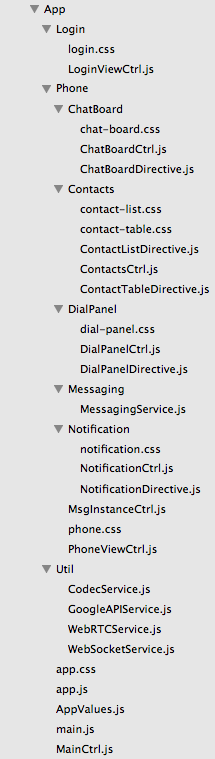
\includegraphics[height=0.45\textheight,natwidth=610,natheight=642]{figs/angularjs_structure.png}
  	\caption{Prototype Application AngularJs Files}
  	\label{fig:angularjs_structure}
\end{figure}

\end{appendices}
